\documentclass[11pt]{article}
\usepackage{geometry}  
%\usepackage[margin=1cm]{geometry}
\usepackage{pgfgantt}
\usepackage{graphicx}
\usepackage{xcolor}
%\usetikzlibrary{positioning}

\ganttset{group/.append style={orange},
milestone/.append style={red},
progress label node anchor/.append style={text=red}}    



% See geometry.pdf to learn the layout options. There are lots.
\geometry{letterpaper}                   % ... or a4paper or a5paper or ... 
%\geometry{landscape}                % Activate for for rotated page geometry
%\usepackage[parfill]{parskip}    % Activate to begin paragraphs with an empty line rather than an indent
\usepackage{graphicx}
\usepackage[colorinlistoftodos]{todonotes}
\usepackage{amssymb}
\usepackage{epstopdf}
\usepackage[english]{babel}
\usepackage{placeins}
\usepackage{tikz}
\usepackage{pgf}
\usepackage{inputenc}
\usetikzlibrary{shapes,arrows}
\usetikzlibrary{automata,positioning}     
\usepackage{listings}
\usepackage{smartdiagram}
\usepackage{tocstyle}
\usetocstyle{standard}



\lstset
{ %Formatting for code in appendix
    language = C,
    basicstyle=\footnotesize,
}   

\tikzset{
    state/.style={
           rectangle,
           rounded corners,
           draw=black, very thick,
           minimum height=2em,
           inner sep=2pt,
           text centered,
           },
}
\DeclareGraphicsRule{.tif}{png}{.png}{`convert #1 `dirname #1`/`basename #1 .tif`.png}
\begin{document}
\begin{titlepage}

\newcommand{\HRule}{\rule{\linewidth}{0.5mm}} % Defines a new command for the horizontal lines, change thickness here

\center % Center everything on the page
 
%----------------------------------------------------------------------------------------
%	HEADING SECTIONS
%----------------------------------------------------------------------------------------

\textsc{\LARGE George Mason University}\\[1.5cm] % Name of your university/college


%----------------------------------------------------------------------------------------
%	TITLE SECTION
%----------------------------------------------------------------------------------------

\HRule \\[0.4cm]
{ \huge \bfseries Implementing OTA Updates for an IoT Security Device}\\[0.4cm] % Title of your document
\LARGE{\textbf{Design Document}}
\HRule \\[1.5cm]
 
%----------------------------------------------------------------------------------------
%	AUTHOR SECTION
%----------------------------------------------------------------------------------------
\begin{minipage}{0.4\textwidth}
\begin{flushleft} \large
\emph{Authors:}\\
Gerson \textsc{Dalton Cardozo} \\
M. Sohail \textsc{Iqbal} \\ 
Aneesh \textsc{Malhotra} \\ 
Mohamed \textsc{Nur} \\ 
Ryan \textsc{Thomas} % Your name 
\end{flushleft}
\end{minipage}
~
\begin{minipage}{0.4\textwidth}
\begin{flushright} \large
\emph{Supervisor:} \\
Dr. Jens-Peter \textsc{Kaps} % Supervisor's Name
\end{flushright}
\end{minipage}\\[2cm]

% If you don't want a supervisor, uncomment the two lines below and remove the section above
%\Large \emph{Author:}\\
%John \textsc{Smith}\\[3cm] % Your name

%----------------------------------------------------------------------------------------
%	DATE SECTION
%----------------------------------------------------------------------------------------

{\large \today}\\[2cm] % Date, change the \today to a set date if you want to be precise

%----------------------------------------------------------------------------------------
%	LOGO SECTION
%----------------------------------------------------------------------------------------

\includegraphics{watermark2.jpg}\\[1cm] % Include a department/university logo - this will require the graphicx package
 
%----------------------------------------------------------------------------------------

\vfill % Fill the rest of the page with whitespace

\end{titlepage}
\clearpage
\tableofcontents
\clearpage
\section{Executive Summary}

This project will build upon a previous ECE 492 project \textit{FPGA Enhanced Wireless Sensor Node for IoT Applications}. The project sought to use an FPGA to enhance the security of a wireless sensor node network while maintaining low power consumption. The network that this was implemented on was an in-home security system, which detects motion using an IR sensor on a node, and sends a picture of the intruder to the user via the gateway. Security can be an issue in wireless sensor networks and it may be necessary to update the private key of compromised node or update the firmware of a node to enhance its performance and functionality. The most efficient and inexpensive way to distribute such an update to many users without having to dismantle the system is over-the-air (OTA). In this process a manufacturer will distribute a secure update to its users and the system will update its own firmware. Our goal in this project is to provide OTA update capability to the in-home security system developed by the previous group. 
\clearpage
\section{Approach}
\subsection{Motivation}

Many IoT devices now use wireless-sensor networks in which a user is able to control several devices called "nodes" through a single device called a "gateway". These kinds of networks are used in many popular smart home devices such as Google's Nest and Phillips Hue, most of which already provide OTA update capability. Additionally, security for these networks is becoming a concern. Wireless sensor networks are often deployed to monitor and respond to events occurring in the environment and are meant to be left unattended, making them susceptible to a variety of attacks \cite{sen_security_2013}. With the versatile capabilities of FPGA's, we see many researchers using FPGA's to enhance the capabilities of wireless sensor networks, including security \cite{g_elliptic_2016}. As FPGA's make their way into more wireless sensor networks, we will need to be able to be able to equip them with OTA update capability. Our goal is to provide this capability to our network that uses an FPGA for enhanced security. 


\subsection{Problem Analysis}
The problem we face is to be able to provide OTA updates to the node of the previous system (Figure 1). Since the node is not directly connected to a computer, we must be able to reprogram the node using only the existing hardware on the node. Additionally, the node consists of an MSP432 microcontroller and an Actel IGLOO FPGA. Updating the security features such as the private key and the algorithm on the FPGA will require us to be able to reprogram the FPGA remotely. Likewise, updating the firmware and capabilities of the microcontroller will require us to be able to reprogram the MSP432 remotely. 

\begin{figure}[!ht]
\centering
\includegraphics[scale = 0.35]{schematic1.png}
\caption{Top Level Diagram of Camera Security System}
\end{figure}
\FloatBarrier


\subsection{Solution}
Our solution to this problem is to redesign the system to be able to request updates from an external sever, download the update to the Gateway, push the update to the MSP432 via the XBee, and allow the MSP432 to reprogram both itself and the FPGA through a bootloader. The update will simply consist of a .zip file that consists of a YAML file, the updated code, and some header information. Our goal is to be able to parse the update on the Gateway, and send bootloader commands to the node. The MSP432 on the node will then use these commands to reprogram its own program memory, as well as interface to and reprogram the FGPA. 


\subsection{Requirements Specifications}

\begin{itemize}
\item External Server 
\begin{itemize}
\item Contains secure signature and contains update ?les.
\item Stores user data collected from the node such as images.
\end{itemize}
\item Update
Contains a .zip file with a YAML ?le as well as the source code.
The YAML file will have an MSP432 and FPGA section, and will be converted to bootloader commands.
\item Phone
Provides interface to user
Checks for and initiates updates
Allows for rekeying and initiating capture from the node camera.
\item Gateway
\begin{itemize}
\item Main system component
\item Contains a BeagleBone Black running Linux and an XBee to communicate with the node
\item Parses YAML \text{?le}, and maps it to bootloader commands for the MSP432.
\item Takes in data from the node and makes it accessible to the user.
\end{itemize}
\item Node
\begin{itemize}
\item Secondary system component
\item Contains an MSP432, Actel IGLOO FPGA, an XBee, an ArduCam v5 5MP camera, and an IR sensor.
\item The MSP432 controls all other components and will have the capability to reprogram itself and the FPGA.
\item The node will capture an image and send it back to the Gateway.
\end{itemize}
\end{itemize}

\subsection{Top-Level Design} 
\begin{figure}[!ht]
\centering
\includegraphics[scale = 0.4]{BlockDiagram.jpg}
\caption{The camera security system no longer uses Dropbox, but rather a server to host the updates.}
\end{figure}
\FloatBarrier


\begin{enumerate}
\item The server contains a file with the version number and location of an update. 
\item The user compares the version number of the update to that of the system.
\item If the version numbers do not agree, the user will have the option to begin an update. 
\item The Gateway will request the complete update, process it, push the the update and appropriate MSP432 commands to the node.
\item MSP432 will receive the update from the Gateway as well as instructions for reprogramming itself and the FPGA. This will be done via Bootloader commands. 
\end{enumerate}
\FloatBarrier

The following diagram depicts this workflow. \vspace{2em}
\begin{figure}[!ht]
\centering
\smartdiagram[flow diagram:horizontal]{Update is available,User Accepts Update ,
  Gateway Requests Update, Gateway Processing, XBee Link, MSP432 Bootloader}
  \caption{Update Workflow}
 \end{figure}


\FloatBarrier


\subsection{Alternative Designs}

\subsubsection{Dropbox}
We had initially decided to use Dropbox as a cloud storage system. Since the gateway is not a member of the local area network, this would have made communication between the Android device and the gateway to be much simpler. This communication, however, is much slower. Additionally a company pushing a firmware update to a user will not typically have access to a user's Dropbox account. A user can also accidentally delete important configuration files such as the ones used for rekeying, making it less reliable and less realistic than a dedicated server. For these reasons, we decided to use a dedicated web server for distributing updates and storing data. 

\subsection{FPGA Programming}
There are many ways about which we can program the ACTEL IGLOO Nano using a microcontroller. One method was rather simple, and involved using a power FET to control the different operating modes, but this component is rather 

\begin{figure}[!ht]
\centering
\includegraphics[scale = 0.35]{opmodes.png}
\caption{Different Operating Modes of the Actel IGLOO Nano}
\end{figure}

\section{System Architecture}


\subsection{Architecture with Pseudo-Code}


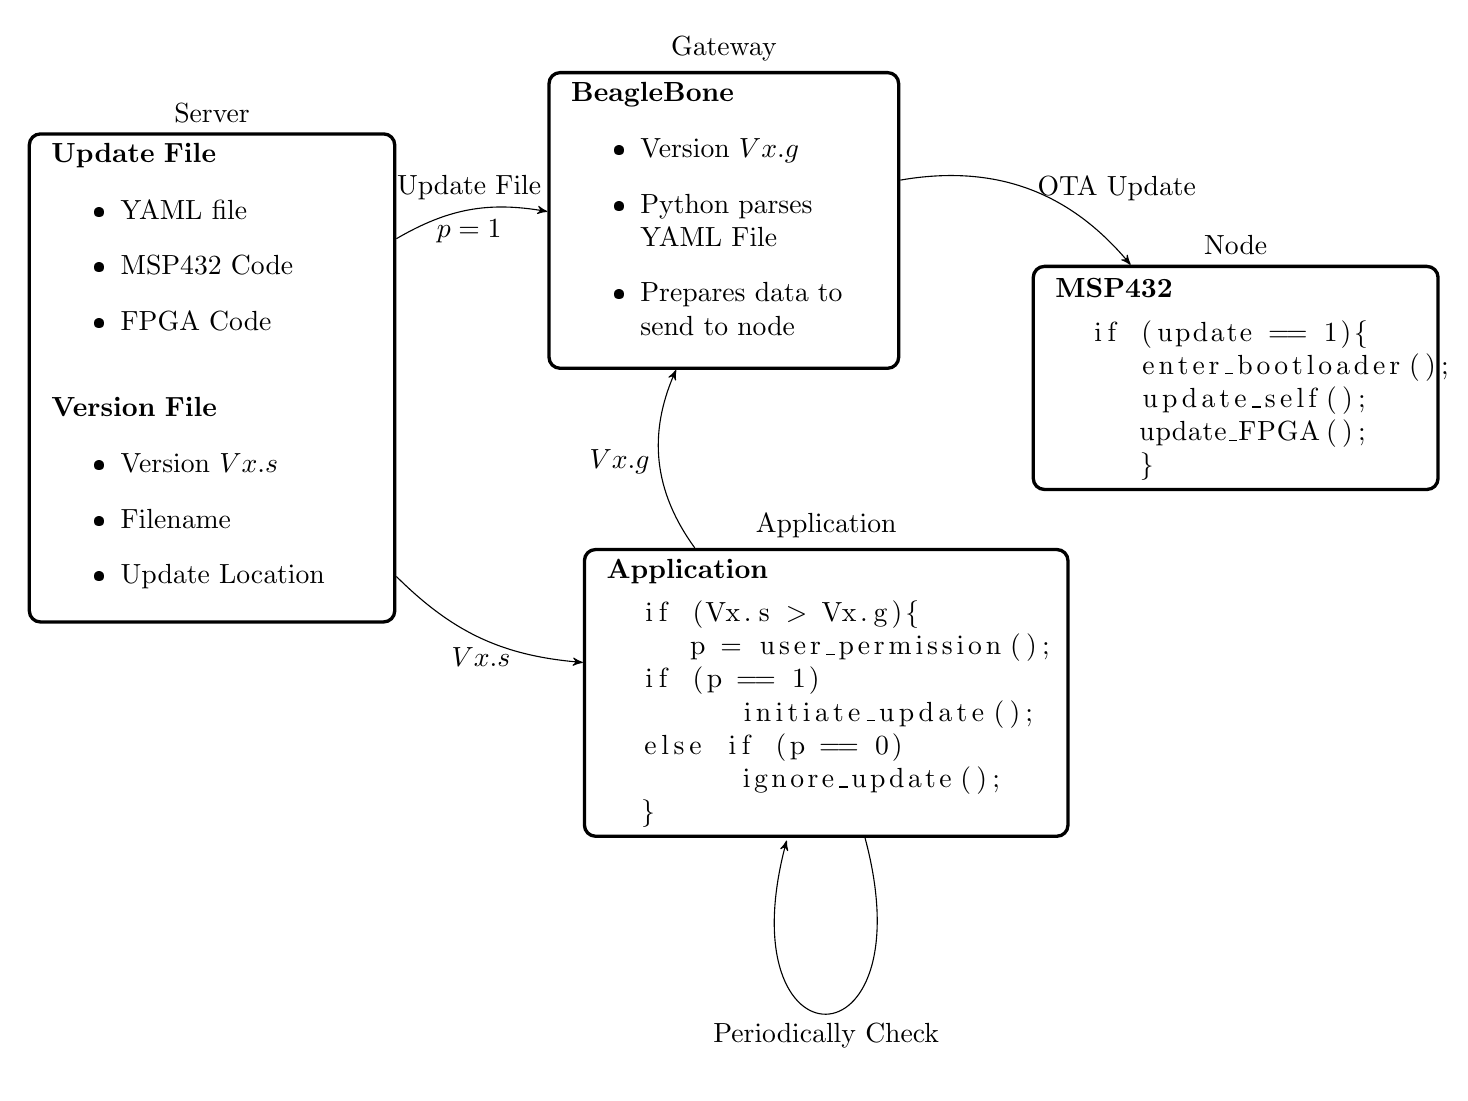
\begin{tikzpicture}[->,>=stealth']

 % Position of QUERY 
 % Use previously defined 'state' as layout (see above)
 % use tabular for content to get columns/rows
 % parbox to limit width of the listing
 \node[state, text width = 4.5cm] [label=Server](SERVER) 
 {\begin{tabular}{l}
  \textbf{Update File}\\
  \parbox{4cm}{\begin{itemize}
   \item YAML file
   \item MSP432 Code
   \item FPGA Code
  \end{itemize}
  }\\[4em]
  \textbf{Version File}\\
  \parbox{5cm}{\begin{itemize}
   \item Version $Vx.s$
   \item Filename
   \item Update Location
  \end{itemize}
  }
 \end{tabular}};
  
 % State: ACK with different content
 
 
 
 \node[state,    	% layout (defined above)
  text width=3cm, 	% max text width
  yshift=2cm, 		% move 2cm in y
  right of=SERVER, 	% Position is to the right of QUERY
  node distance=6.5cm, 	% distance to QUERY
  anchor=center,
  text width = 4.3cm][label = Gateway] (GATEWAY) 	% posistion relative to the center of the 'box'
 {%
 \begin{tabular}{l} 	% content
  \textbf{BeagleBone}\\
  \parbox{4cm}{
  \begin{itemize}
  \item Version $Vx.g$
  \item Python parses YAML File
  \item Prepares data to send to node
  \end{itemize}
  }
 
  
 \end{tabular}
 };
 
 % STATE APPLICATION
 \node[state,
  below of=GATEWAY,
  yshift=-5cm,
  xshift = 1.3cm,
  anchor=center,
  text width=6cm] [label = Application](APPLICATION) 
 {%
 \begin{tabular}{l}
  \textbf{Application}\\

  \begin{lstlisting}
  if (Vx.s > Vx.g){
     p = user_permission();
  if (p == 1)
  	initiate_update();
  else if (p == 0)
  	ignore_update();
  }
  
  \end{lstlisting}

 \end{tabular}
 };

 % STATE EPC
 \node[state,
  right of=GATEWAY,
  node distance=7cm,
  anchor=center, text width = 5cm, yshift = -2cm,xshift = -.5cm] [label = Node](NODE) 
 {%

 \begin{tabular}{l}
  \textbf{MSP432}\\

  \begin{lstlisting}
  if (update == 1){
     enter_bootloader();
     update_self(); 
     update_FPGA();
     }
  \end{lstlisting}


 \end{tabular}
 };

 % draw the paths and and print some Text below/above the graph
 \path (SERVER) 	edge[bend left=20]  node[anchor=south,above]{Update File}
                                    node[anchor=north,below]{$p = 1$} (GATEWAY)
 (SERVER)     	edge[bend right=20] node[anchor=south,below]{$Vx.s$} (APPLICATION)
 (GATEWAY)       	edge  [bend left]                      node[anchor=north,right]{OTA Update}(NODE)
 (APPLICATION)  	edge[loop below]    node[anchor=north,below]{Periodically Check} (APPLICATION)
 (APPLICATION)  	edge[bend left]         node[anchor = left, left]{$Vx.g$} (GATEWAY);

\end{tikzpicture}



\subsection{Architecture 2}


\begin{figure}[!ht]
\centering
\includegraphics[scale = 0.55]{system2.png}
\caption{The system architecture with all components and functionality}
\end{figure}
\FloatBarrier

\subsection{Node State Diagram}

The following is the state diagram of the node in the IoT Device. 


\begin{figure}[!ht]
\centering
\includegraphics[scale = 0.35]{nodestate.png}
\caption{State diagram for the node}
\end{figure}
\FloatBarrier
\subsection{Gateway state diagram}

\begin{figure}[!ht]
\centering
\includegraphics[scale = 0.35]{nodestate.png}
\caption{State diagram for the node}
\end{figure}
\FloatBarrier
\subsection{Gateway State Diagram}

\begin{figure}[!ht]
\centering
\includegraphics[scale = 0.35]{gatewaystate.png}
\caption{State diagram for the gateway}
\end{figure}

\FloatBarrier

\section{Background Information}

The project we are building is an addition to a previous Senior Design Project the background knowledge required can be broken up into the following sections:

\subsection{Current System}

\begin{itemize}

\item Memory 
\begin{itemize}
\item Current Flash Main Memory usage is 7.5KB based on current program 
\item Current SRAM usage is 2KB for the program and 60KB for the photo 
\item Current total SRAM Usage is 62 KB with 8KB of SRAM remaining 
\end{itemize}
\item Serial Communication 
\begin{itemize}
\item eUSCI\_A Modules 
\item UART is utilized by the Xbee S2C 
\item eUSCI\_B Modules 
\item GPIO is used be Arducam OV2640, IGLOO nano, and HC-SR501 PIR MOTION DETECTOR 
\item SPI is used be Arducam OV2640 
\end{itemize}
\end{itemize}
 
\subsection{PCB Design}
For the PCB we will need to optimize the design for testing. We will need to make each component accessible for testing the power consumption of each component (using a multimeter). We will use KiCad for the PCB design, and will need to learn to use KiCad. 

\subsection{Server}

We will be using Node.js to implement an HTTPS sever that can store the update and some user data. Since this will be used instead of Dropbox, we will have to use the server to store pictures sent from the node to the gateway, since the phone is unable to connect directly to the BeagleBone. We can implement this as a website where images are stored. 


\subsection{FPGA/MSP432}
We will also require a profound knowledge of coding C for programming the MCU that controls the node. Additionally, Linux bAdditash scripting commands in order for the gateway to push and pull data from the node. On a hardware level there will need to be able to set the clock speeds on the MCU as well configuring pins for serial communication via SPI, I2C, UART. Data on the MCU is handled in 1 byte chunks. And the data transfer speeds are determined by the MCU’s clock speeds. We will require knowledge of the STAPL player for programming the IGLOO. 
\subsection{Security}


Keeping the system secure is one of our main goals. In the system that we have so far, we are using the following security protocols
\begin{itemize}
    \item Security Protocols Used: 
    
    \begin{itemize}
       \item  Transport Layer Security (TLS) 
        \item 128 – bit AES Encryption 
        \item Produced by the elliptic curve scheme on BeagleBone and FPGA 
        \item The FPGA has a 128 bit AES encryption within itself to protect data transfer 
    \end{itemize}
\end{itemize}


\subsubsection{Elliptic Curve Cryptography}

The previous project implemented a security verification scheme based on elliptic curve cryptography. This is implemented as asymmetric cryptography where we generation a session key. This session key is used for securing the communication between the gateway and the node via ZigBee. An elliptic curve is a function of the form 

\[y^2 = x^3 + ax + b \]

under a finite field, such as the $\mathbb{Z}$ (mod p)

\begin{figure}[!ht]
\centering
\includegraphics[scale = 0.35]{ecurve.png}
\caption{Elliptic Curve for $a = 1$ and $b = 2$}
\end{figure}

We can use these curves to implement a security algorithm in which we use elliptic curve arithmetic to generate a session key. We define the a group operation $g$ on elliptic curves. The BeagleBone's private key will be some number $a$, and the private key of the Node will be some number $M_{b}$ The BeagleBone will establish a session key by performing the group operation $a$ times on the public key of the node resulting in $S = M_b^a$, where $S$ is the session key. The Node verifies the session key in the FPGA, which is already programmed to handle heavy arithmetic, and forwards it to the ZigBee as the key used for symmetric AES encryption. 



\subsubsection{Securing the Update}

The update will be secured on the server using TLS (Transport Layer Security), by having the BeagleBone request the udpate from only the server's certificate and public key. After having this implemented, the update will be secured through the session key that was already established. 


\section{Prototyping Progress}

\subsection{List of Acquired Components}

\begin{enumerate}
    \item Actel IGLOO Nano
    \item MSP432 Trainer Board
\end{enumerate}

We still need to buy the camera, IR sensor, BeagleBone, and XBee devices.

\subsection{Current Working Components}

We currently have an HTTP server built in Python, but we will rebuild it using Node.js to provide a better user interface. Additionally, we have the FPGA side working. We have a version of the app running as well.


\subsection{Testing Plans}
We plan on testing the system by adding a noticeable change to the MSP432 code such as toggling the state of an LED. Testing the programmability of the FPGA will be done in a similar way.These experiments are simple, don't involve as much writing as much code, and will allow us to focus on testing programmability.


\subsection{Task for Next Semester} 


\scalebox{0.45}{
\begin{center}
     \begin{ganttchart}[%Specs
     y unit title=0.5cm,
     y unit chart=0.7cm,
     vgrid,hgrid,
     title height=1,
%     title/.style={fill=none},
     title label font=\bfseries\footnotesize,
     bar/.style={fill=blue},
     bar height=0.7,
%   progress label text={},
     group right shift=0,
     group top shift=0.7,
     group height=.3,
     group peaks width={0.2},
     inline]{1}{45}
    %labels
    \gantttitle{IOT Security Device Semester 2}{45}\\  % title 1
    \gantttitle[]{Weeks 1-7 }{21}                 % title 2
    \gantttitle[]{Weeks 8-15}{24} \\              
    \gantttitle{W1}{3}                      % title 3
    \gantttitle{W2}{3}
    \gantttitle{W3}{3}
    \gantttitle{W4}{3}
    \gantttitle{W5}{3}
    \gantttitle{W6}{3}
    \gantttitle{W7}{3} 
    \gantttitle{W8}{3}
    \gantttitle{W9}{3}
    \gantttitle{W10}{3}    
    \gantttitle{W11}{3}
    \gantttitle{W12}{3}
    \gantttitle{W13}{3}     
    \gantttitle{W14}{3}      
    \gantttitle{W15}{3}\\
    % Setting group if any
    \ganttbar[progress = 100,inline=false]{Server Development}{1}{15}\\
    \ganttbar[progress = 10, inline=false]{MSP432 Programming FPGA}{1}{30}\\
    \ganttbar[progress = 30, inline = false]{Fixing Application}{21}{28}\\
    \ganttbar[progress = 0, inline = false]{Create standard for the update/security}{1}{20}\\
    \ganttbar[progress = 00, inline = false]{Implement Packetization of Update/Data}{2}{9}\\
    \ganttbar[progress = 00, inline = false]{Testing/Debugging}{40}{45}
   
\end{ganttchart}
    \caption{Gantt diagram for ECE 493}
\end{center}
}
\FloatBarrier

\subsection{Task List}

\begin{enumerate}
    \item FPGA Programming 
    \begin{enumerate}
        \item Simulate a JTAG interface to program the FPGA.
        \item Once MSP432 works, test the model and see if we can change the FPGA code to toggle an LED
    \end{enumerate}
    \item MSP432 Bootloader
    \begin{enumerate}
        \item Setup MSP432 Bootloader
        \item Use an external signal to activate bootloader mode 
        \item Test bootloader commands by rewriting a block of program memory. 
    \end{enumerate}
    
    \item Server
    \begin{enumerate}
        \item Build HTTP server using Node.js
        \item Build a website to display images on
        \item (Theoretically) get a certificate and implement an HTTPS server. 
    \end{enumerate}
    \item Update
    \begin{enumerate}
        \item Finalize update design, and make sure everybody knows what the update will looks like
        \item Build a parser using Python on the BeagleBone that can read the update, and send information to the node. 
    \end{enumerate}
\end{enumerate}
\bibliographystyle{apalike}
\bibliography{refs}



\end{document}  